% \clearpage
\appendix
\renewcommand{\tablename}{Appendix Table}
\setcounter{table}{0}
\renewcommand{\thetable}{A\arabic{table}}
\renewcommand{\tablename}{Appendix Table}
\setcounter{algorithm}{0}
\renewcommand{\thealgorithm}{A\arabic{algorithm}}
\renewcommand{\figurename}{Appendix Figure}
\setcounter{figure}{0}
\renewcommand{\thefigure}{A\arabic{figure}}
\setcounter{equation}{0}
\renewcommand{\theequation}{A\arabic{equation}}
\section{Full Notations and operators}
We summarize the notations and operators used
in this work in \cref{tab: notations}.

\begin{table}[t!] 
% \addtolength{\tabcolsep}{-2pt}
% \footnotesize
   \begin{center}
   \vspace{-0em}
       \caption{Summary of Notations}\label{tab: notations}
       \vspace{-0em}
     \begin{tabular}{c|l}
        \toprule[1.0pt]
        Notation & Description \\
        \midrule
        $\db$ &  The database \\
        $\dbtab$ &  The data tables in the database \\
        $\dbtabrowsize$ & The number of rows in table $\dbtab$ \\
        $\dbtabcolsize$ & The number of columns in table $\dbtab$ \\
        $\dbquery$  & The SQL query.\\
        $\dbabsquery$  & The number of predicates in query $\dbquery$.\\
        $\mathcal{M}$ &  The data analysis model\\
        $\algoweight$ & The parameters in data analysis model \\
        \midrule
        $\lambda$ & The security parameter\\
        $p$       & The plaintext modulus \\
        $q$       & The ciphertext modulus for $\lwe$\\
        $Q$       & The ciphertext modulus for $\rlwe$\\
        $Q'$       & The ciphertext modulus for $\rgsw$\\
        $n$       & The lattice dimension for $\lwe$\\
        $N$       & The lattice dimension for an $\rlwe$\\
        $N'$       & The lattice dimension for an $\rgsw$\\
        $l$       & The number of $\rlwe$ in $\rgsw$ \\
        % $\mathbb{Z}_q$ & The ring of integers modulo $q$ \\
        $\mathbb{Z}_{q}^{n}$ & The set of n-vectors over $\mathbb{Z}_q$ \\
        % $\mathbb{Z}[X]$ & The polynomial ring over $\mathbb{Z}$ \\
        % $\mathbb{Z}_{q}[X]$ & The polynomial ring over $\mathbb{Z}_q$ \\
        $R$ & The cyclotomic ring   $\mathbb{Z}[X]/(X^N+1)$\\
        $R_{Q} $ & The cyclotomic ring $\mathbb{Z_{Q}}[X]/(X^N+1)$ \\
        $\chi$ & The noise distribution \\
        $\Delta$ & The scaling factor \\
        $\mathbf{a}$ & An element in vector domain \\
        $\mathbf{a}_i$ & The i-th element of $\mathbf{a}$ \\
        $ \Tilde{a} $ & An element in polynomial ring \\
        $ \Tilde{a}_i $ & The i-th coefficient of $\Tilde{a}$ \\
        $ \mathbf{A} $ & An element in matrix domain \\
        $\mathfrak{d} $ & The number of the leaf nodes\\
        % $ \hat{a} $ & The NTT-domain of element $a$ \\
        \midrule
        \multirow{2}{*}{$ \lwe^{n, q}_{\bs}(m) $} & An LWE ciphertexts encrypting $m$ \\
        & with parameters $(n, q)$ and secret $\bs$\\
        \multirow{2}{*}{$ \rlwe^{N, Q}_{\tts}(\ttm) $} & An RLWE ciphertexts encrypting $\ttm$ \\
        & with parameters $(N, Q)$ and secret $\tts$\\
        \multirow{2}{*}{$ \rgsw^{N', Q'}_{\Tilde{\bs}}({\bf{m}})$} & An RGSW ciphertext encrypting
        {\bf{m}} \\
        & with parameters $(N', Q')$ adn secret $\Tilde{\bs}$ \\
        $\diamond $ & Homomorphic matrix-vector multiplication\\
        %$ +, -, \cdot$ & Addition, subtraction and multiplication \\
        $ \cmux $  & Homomorphic selector~\cite{DBLP:journals/joc/ChillottiGGI20}\\
        $ \pbs  $ &  Programmable bootstrapping~\cite{DBLP:conf/asiacrypt/tfhepbs} \\
        $ \homgate$  & Homomorphic gate~\cite{DBLP:conf/eurocrypt/DucasM15, DBLP:journals/joc/ChillottiGGI20}\\
        $\bar{ct}$ & The NOT gate result of $ct$ \\
        \multirow{2}{*}{$\sei$} & Converting RLWE to LWEs \\
                & (a.k.a, sample extract index~\cite{DBLP:journals/joc/ChillottiGGI20}) \\
        \multirow{2}{*}{$\repack$} & Converting LWEs to RLWE \\
        & (a.k.a, repack~\cite{pegasus,conversionhaochen}) \\
        \multirow{2}{*}{$\cb$} & Converting LWE to RGSW \\
        & (a.k.a., circuit bootstrapping~\cite{DBLP:journals/joc/ChillottiGGI20}) \\
        \bottomrule[1.0pt]
     \end{tabular}
   \end{center}
    \vspace{-0em}
\end{table}
\begin{figure*}[t!]
   \begin{center}
    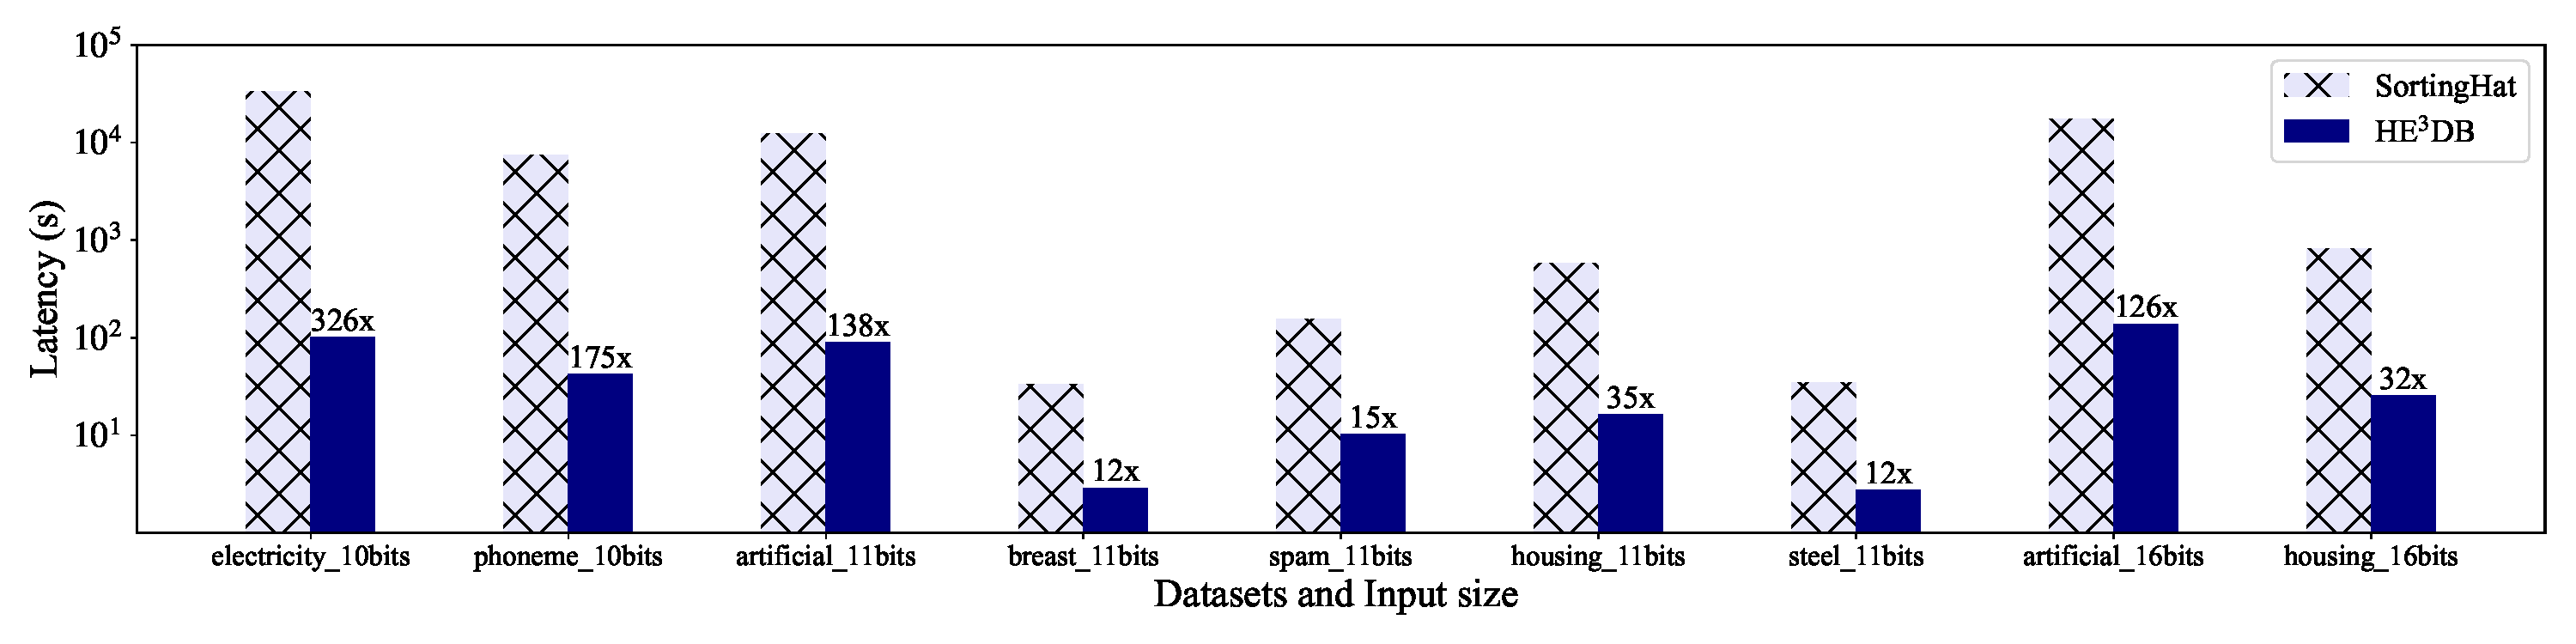
\includegraphics[width=\linewidth]{figure/treebench.pdf}
   \end{center}
    \vspace{-0.5em}
      \caption{Running time of our PTDE algorithm compared to SortingHat~\cite{sortinghat}} 
   \label{fig: homtreebench}
   \vspace{-0.5em}
\end{figure*}

\begin{algorithm}[t!]
    % \tiny
    \caption{\br}
    \label{algo: kHMSB}
    \SetKwInOut{Input}{Input}\SetKwInOut{Output}{Output}\SetKwInOut{Return}{Return}
    \Input{A Test polynomial $\Tilde{v} = v_0 + v_1x + ... + v_{N-1}x^{N-1}$.}
    \Input{An LWE ciphertext $ct = \lwe_{\mathbf{s}}^{n,q}(m) = (b, \mathbf{a})$.}
    \Input{A bootstrapping key $\bBK$, where 
    $\bBK\left[i\right] = \rgsw^{N',Q'}_{\Tilde{s}}(\mathbf{s}_{i})$, for $i \in [1,n]$}
    \Output{A LWE ciphertext $ct_{O} = \lwe_{\mathbf{s}}^{n,q}(v_{m})$.}
    $b \leftarrow \round{\frac{2N}{q}b} $ 
    and $\mathbf{a} \leftarrow \round{\frac{2N}{q}\mathbf{a}_{i}}$. \\
    $\Tilde{v} \leftarrow \mu \cdot (1 + x^2 + x^3 + ... + x^{N-1}) $ \\
    Initialize $ACC \leftarrow X^{-b}\cdot (\Tilde{v}, 0) \in \rlwe_{\Tilde{s}}^{N,Q}(.)$. \\
    \For { $i = 0$ \KwTo $n-1$}
    {
        $ACC \leftarrow \cmux(\bBK_{i}, X^{-\mathbf{a}[i]} \cdot ACC, ACC)$
    }
    $ct_{O} \leftarrow \sei(ACC)[0]$ \\
    \Return{$ct_{O}  
    = \lwe_{\mathbf{s}}^{n,q}(v_{m})$}
\end{algorithm}

\begin{algorithm}[t!]
    % \tiny
    \caption{$\kappa$-bit $\pbshmsb$}
    \label{algo: kHMSB}
    \SetKwInOut{Input}{Input}\SetKwInOut{Output}{Output}\SetKwInOut{Return}{Return}
    \Input{A LWE ciphertext $ct_{I} = \lwe^{n,q}_{\mathbf{s}}(m) 
    = (b, \mathbf{a})$, where $m \ in [0, 2^{k} -1]$.}
    \Input{A constant $\mu = q / 4$.}
    \Input{A bootstrapping key $\bBK$, where 
    $\bBK\left[i\right] = \rgsw^{N',Q'}_{\Tilde{s}}(\mathbf{s}_{i})$, for $i \in [1,n]$}
    \Output{A LWE ciphertext $ct_{O} = \lwe_{\mathbf{s}}^{n,q}(\msb(m))$.}
    % $b \leftarrow \lfloor \frac{2N}{q}b \rceil$ 
    % and $\mathbf{a} \leftarrow \lfloor \frac{2N}{q}\mathbf{a} \rceil$ \\
    $\Tilde{v} \leftarrow \mu \cdot (1 + x^2 + x^3 + ... + x^{N-1}) $ \\
    $ACC \leftarrow \br(\Tilde{v}, ct_I, \mathbf{BK})$ \\
    $ct_{O} = (b', \mathbf{a'}) \leftarrow \sei(ACC)[0]$ \\
    \Return{$ct_{O} = (b' + \mu, \mathbf{a}) 
    = \lwe_{\mathbf{s}}^{n,q}(\msb(m))$}
\end{algorithm}

% \begin{algorithm}[t!]
%     % \footnotesize
%     \caption{\texttt{1-out-of-k-CMUX}}
%     \label{algo: kcmux}
%     \SetKwInOut{Input}{Input}\SetKwInOut{Output}{Output}\SetKwInOut{Return}{Return}
%     \Input{$k$ $(\ge 2)$ LWE ciphertexts
%     $ct_0, ct_1, ...,ct_{k-1}$.}
%     \Input{$k-1$ control signals $C_1, C_2, ..., C_{k-1}$ where $C_t = 
%     \rgsw(1)$ and else are $\rgsw(0)$}
%     \Output{An LWE ciphertext $ct_{O} = ct_t$}
%     Initialize $ACC \leftarrow ct_0$. \\
%     \For{$i = 1$ \KwTo $k - 1$}
%     {
%         $temp_i \leftarrow ct_i - ct_0$ \\
%         $ACC \leftarrow ACC + temp_i \odot C_i$
%     }
%     \Return{$ACC$}
% \end{algorithm}

% \begin{algorithm}[t!]
%     % \tiny
%     \caption{Optimized Homomorphic \texttt{MIN} Aggreagation \texttt{OpHomMINAgg}}
%     \label{algo: ophomminagg}
%     \SetKwInOut{Input}{Input}\SetKwInOut{Output}{Output}\SetKwInOut{Return}{Return}
%     \Input{An RLWE ciphertext of the aggregated column $ct = \rlwe(\Tilde{m}), 
%     \Tilde{m}_i = m_i, i \in \mathbb{Z}_{\dbtabrowsize}$.}
%     \Input{Filtered result $cf=
%     (cf_{1}, cf_{2}, ... ,cf_{\dbtabrowsize})$, where
%     $cf_i = \lwe(f_i)$, $f_i = 0$ or $1$.}
%     \Input{The Pre-defined constant $\lwenan$.}
%     \Input{A bootstrapping key $\bBK$.}
%     \Output{A LWE ciphertext $ct_{O} = \lwe(\dbmin(m_{t_1}, ...,m_{t_f}))$ where
%     $f =  {\textstyle \sum_{i=0}^{\abs{\mathcal{T}}_{r}}}f_i$
%     and $f_{t_1}, f_{t_2}, ..., f_{t_{f}} = 1$.}
%     $\mathbf{ct} = \sei(ct) = (ct_1, ct_2, ...,ct_{\dbtabrowsize})$ \\
%     \For{$i = 1$ \KwTo $\frac{\dbtabrowsize}{2}$}
%     {
%         $c = \homcomp(ct_{2i-1}, ct_{2i}, \leq)$ \\
%         $c_1 = \homgate(cf_{2i-1}, \bar{cf_{2i}}, \reg{AND}) + 
%                \homgate(
%                \homgate(cf_{2i-1}, cf_{2i}, \reg{AND}), c, \reg{AND})$ \\
%         $c_2 = \homgate(cf_{2i}, \bar{cf_{2i-1}}, \reg{AND}) + 
%                \homgate(
%                \homgate(cf_{2i-1}, cf_{2i}, \reg{AND}), \bar{c}, \reg{AND})$ \\
%         $C_1 = \cb(c_1, \bBK)$ \\
%         $C_2 = \cb(c_2, \bBK)$ \\
%         $ct_{2i} = \texttt{1-out-of-3-CMUX}
%         (C_1, C_2, ct_{2i-1}, ct{2i}, \lwenan)$ \\
%     }
%     \For{$i = 2$ \KwTo $\log_{2}{\dbtabrowsize}$}
%     {
%         \For{$j = 1$ \KwTo $2^{\log_{2}{\dbtabrowsize} - i}$}
%         {
%             $ct_{2^{i}j} = \hommin
%             (ct_{2^{i}j-2^{i-1}}, ct_{2^{i}j}, \bBK)$ \\
%         }
%     }
%     \Return{$ct_{O} = ct_{2^{n}}$}
% \end{algorithm}

% \begin{lemma}
%     The output of \cref{algo: ophomminagg} is equal to 
%     \cref{algo: homminagg} and 
%     the number of homomorphic \texttt{CMUX} gates is 
%     $\frac{\abs{\mathcal{T}}_{r}}{2} -1$, 
%     the number of homomorphic \texttt{1-out-of-3 CMUX} gates is 
%     $\frac{\abs{\mathcal{T}}_{r}}{2}$.
%     the number of homomorphic 
%     \texttt{LWEToRGSW} instructions is 
%     $\frac{3\abs{\mathcal{T}}_{r}}{2} -1)$,
%     the number of homomorphic 
%     \texttt{HomCom} instructions is
%     $\abs{\mathcal{T}}_{r}-1$.
%     \label{lemma: ophomminagg}
% \end{lemma}

\section{Proof for Lemma 4.1 and Lemma 4.2}
\begin{proof} \textbf{\cref{lemma: homcomp}}
    First, we prove the correctness of the \cref{algo: homcom}.
    If the comparison operator is $\geq$, 
    the line 2 in \cref{algo: homcom} results 
    $\lwe(\texttt{NOT}(\msb(a-b))$.
    the predicate $a \geq b$ is equal to $\msb(a - b) == 0$.
    If $a \geq b$, the predicate is True, and $\lwe(\texttt{NOT}(\msb(a-b)) = \lwe(1)$. 
    If $a < b$, the predicate is False, and $\lwe(\texttt{NOT}(\msb(a-b)) = \lwe(0)$. 
    Other comparison operators are the same.
    The number of $\pbs$ in \cref{algo: homcom}
    includes the $\pbs$ in $\hmsb$ and $\homgate$.
    From \cref{algo: tkHMSB}, the number of $\pbs$ 
    evaluated in a $tk$-bit ciphertext
    MSB extraction is $2 \times (t - 1) + 1 = 2t - 1$.
    Meanwhile, one $\homgate$ 
    includes one $\pbs$ as we discussed in \cref{pre:he_circuits}.
    Thus, the number of $\pbs$ in \cref{algo: homcom} 
    is $2t-1$ when the comparison operator is $>,<$ and  $2t$  when the comparison operator is $\geq, \leq, ==, \ne$.
\end{proof}

\begin{proof} \textbf{\cref{lemma: homminagg}}
    In \cref{algo: homminagg}, the first for loop (line 2-4)
    includes $\dbtabrowsize$ $\cb$ and $\cmux$, the second for loop (line 5-7)
    contains $2^{\log_{2}{\dbtabrowsize - 1}} + 2^{\log_{2}{\dbtabrowsize - 2 }} 
    + ... + 2^{0} = \dbtabrowsize - 1$ $\hommin$.
    As shown in \cref{algo: hommin}, each $\hommin$ has one $\homcomp$, 
    one $\cb$ and one $\cmux$.
    Therefore, the total number of $\cmux$ gates is $\dbtabrowsize + \dbtabrowsize - 1 = 2\dbtabrowsize - 1$, the whole number of $\cb$ operators is 
    $\dbtabrowsize + \dbtabrowsize - 1 = 2\dbtabrowsize - 1$, the number of 
    $\homcomp$ is $\dbtabrowsize - 1$.
    \label{proof: homminagg}
\end{proof}


 % \begin{proof} \textbf{\cref{lemma: ophomminagg}}
 %     We
 %     \label{proof: ophomminagg}
 % \end{proof}


\section{Additional Comparisons against SAGMA}
\begin{figure}[t!]
   \begin{center}
    \begin{subfigure}[b]{0.25\textwidth}
    \centering
    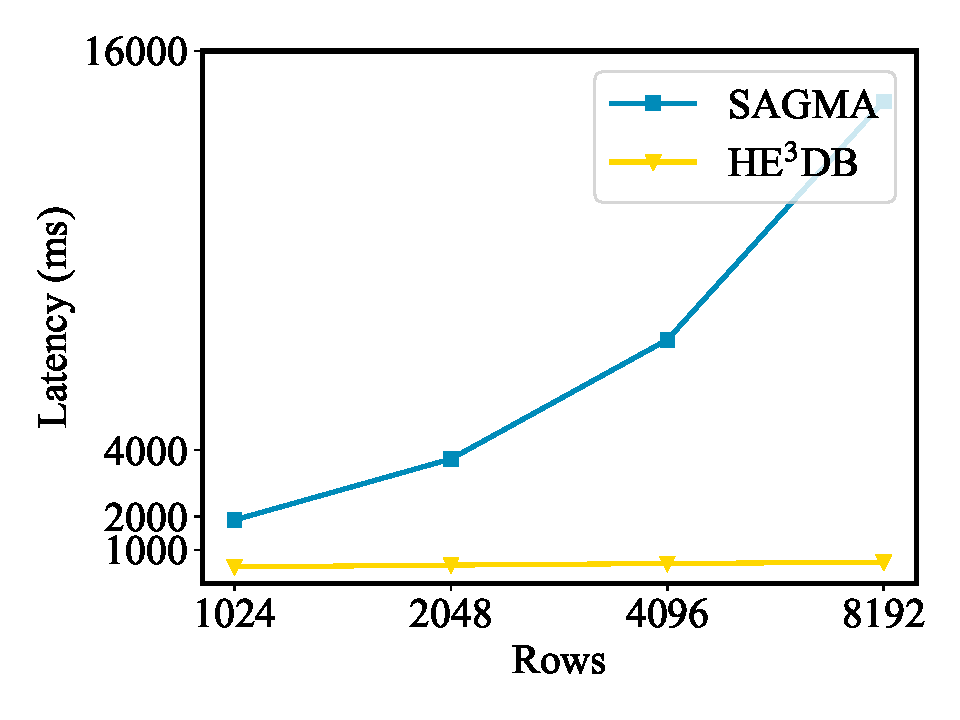
\includegraphics[width=\linewidth]{figure/benchmark_count.pdf}
    % \vspace{-1em}
    \caption{$\dbcount$}
    \label{fig: aggcount}
    \end{subfigure}%
    % \hfill
    \begin{subfigure}[b]{0.25\textwidth}
    \centering
    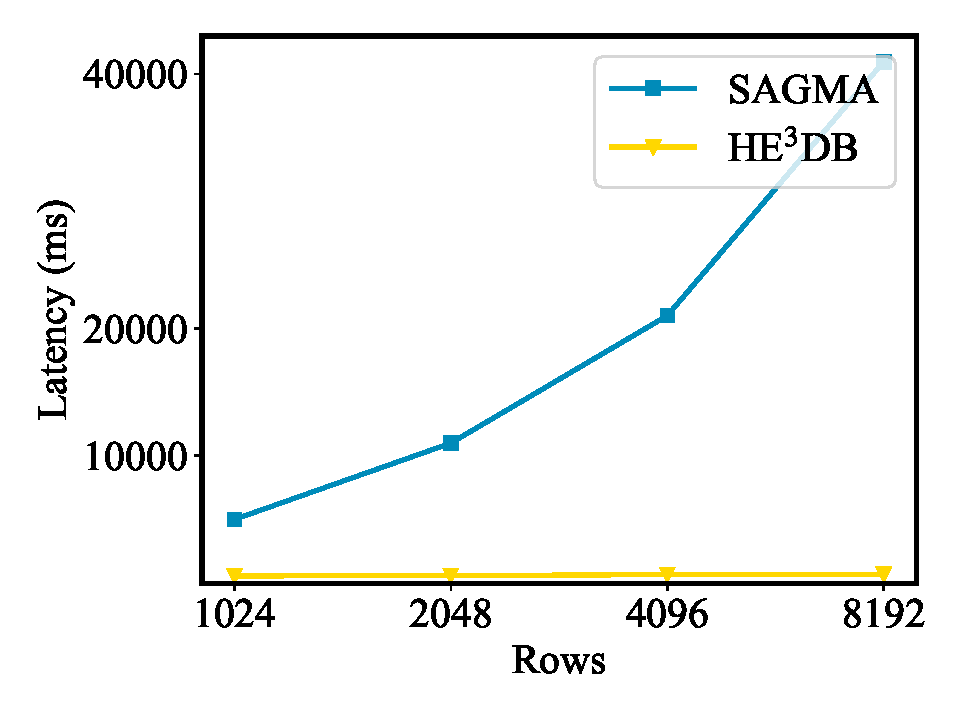
\includegraphics[width=\linewidth]{figure/benchmark_sum.pdf}
    % \vspace{-1em}
    \caption{$\dbsum$}
    \label{fig: aggsum}
    \end{subfigure}%
    % \hfill
   \end{center}
    % \vspace{-1em}
      \caption{Comparison with SAGMA~\cite{sagma} on aggregation function $\dbcount$ and $\dbsum$.} 
      \Description{Comparison with SAGMA~\cite{sagma} on aggregation function $\dbcount$ and $\dbsum$.}
   \label{fig: aggbench}
   % \vspace{-0.5em}
\end{figure}
As SAGMA~\cite{sagma} only uses HE 
in its aggregation process,
we only compare \NAME with SAGMA on the arithmetic aggregation tasks.
As shown in \cref{fig: aggbench}, we can obtain $23\times$ and 
$58\times$ faster in $\dbcount$ and $\dbsum$ operations on a 8192-row database, respectively.

\section{Evaluating Private Outsourced Decision Tree}
\begin{algorithm}[t!]
\caption{\texttt{PDTEval} based on $\homcomp$}
\label{algo:pdte}
 \SetKwInOut{Input}{Input}\SetKwInOut{Output}{Output}\SetKwInOut{Return}{Return}
\Input {Private decision tree Model $\mathcal{CM}$=\{$(ct_0, ..., ct_{2\mathfrak{d}-2}),\\ (a_0, ..., a_{2\mathfrak{d}-2}),(cw_0, ..., cw_{\mathfrak{d}-1})$\}}
\Input {Query results $\mathcal{CR}$= $(cr_0, cr_1, ..., cr_{\lvert G \rvert})$}
\Output{ $\mathfrak{d}$ values of leaves: ${z_0}, ..., {z_{\mathfrak{d}-1}}$}
\State Initialize root value $v_0$ as ${\rm LWE}^{n,q}_{\mathbf{s}}(1)$\\
\State Initialize other node value $v_j$ as ${\rm LWE}^{n,q}_{\mathbf{s}}(0), j \in \left\{ 1, ..., 2\mathfrak{d}-2 \right\}$\\
\For {$i = 0$ \KwTo  $2\mathfrak{d}-2$}{
    \State${cb_i}\leftarrow\; \texttt{HomComp}({cr_{a_i}},{ct_i},\ge )$
}
\For { $i = 1$ \KwTo $\log{\mathfrak{d}}$}{
\For {$j = 0$ \KwTo   $2^{i-1}-1$}{
\State$v_{2^i + 2*j }\leftarrow\; \texttt{HomGate}({cb_{2^{i-1}-1 + j}},v_{2^{i-1}-1 + j}, \texttt{AND})$
\State$v_{2^i + 2*j- 1}\leftarrow\; v_{2^{i-1}-1 + j} - v_{2^i + 2*j}$}
}
\For { $i = 0$ \KwTo $\mathfrak{d}-1$}{
\State${z_i}\leftarrow\; v_{2^{\log \mathfrak{d}}-1+i}$}
\Return{${z_0},...,{z_{\mathfrak{d}-1}}$}
\end{algorithm}
A private decision tree model $\mathcal{CM}$ includes the encryption of threshold $ct_i$, the attribute index $a_i$ and the encryption of label $cw_i$. \cref{algo:pdte} shows our PDTE algorithm, which involves the following steps:\\
\step{Line 1-2, Initialization}:
Server initializes the value of each node as the encryption of 0, denoted by $v_j$ for all $j \in \{0,...,\mathfrak{d}-2\}$, except the root, denoted by $v_0$,  which contains the encryption of 1.\\
\step{Line 3-5, Comparison}:
For each decision node $i$, server computes the Homomorphic Comparison function ${cb_i} \leftarrow [cr_{a_{v}} \ge ct_i}]$, we denote the controller bit of each node by ${cb_i}$ corresponding to the node $i$
for $i$ $\in \{0,...,\mathfrak{d}-2\}$.\\
\step{Line 6-10, Traversal}:
Then the server moves root value ${v_0}$ from the root to a desired leaf. The path depends on the controller bits on each node. Take node $i$ as an example, if node $i$ has value ${v_i}$ and the controller bit of $i$ is ${cb_i}$, the value of the left child node (denoted by ${v_{Lci}}$)and the right child node (denoted by ${v_{Rci}}$) are compute as ${v_{Rci}} = \texttt{HomAND}({cb_i}, {v_i})$, 
${v_{Lci}} = {v_i} - {v_{Rci}}$. After traversal, the value of the root (which is the encryption of 1) is copied to the desired place.\\
Finally, only one leaf has a value which is the encryption of 1, we can easily get this unique label value.\\

{\bf{Evaluation Results}}: As shown in \cref{fig: homtreebench}, 
since SortingHat~\cite{sortinghat} does not target
on evaluating private decision under a secure computation outsourcing setting, we can achieve
up to 300$\times$ speedup using \cref{algo:pdte}.


% The algorithm involves the following steps:
% First, server computes the homomorphic comparison function between threshold value and correspond input attribute for each decision node $i$, restore the comparison result as controller bits ${cb_i}$. Second, server traverses the tree, moves root value $v_0$ from the root to a desired leaf. The path depends on the controller bits on each node. Take node $i$ as an example, if node $i$'s controller bits ${cb_i}$ is the encryption of 1, then copy the node value to its right child  and the left child node value becomes the encryption of 0. Otherwise, vice versa. After traversal, the value of root (which is the encryption of 1) is copied to the desired place. Finally we use homomorphic multiplication to obtain the analysis result.
%For the detailed \texttt{PDTEval} description, see the appendix.

% In \cref{eva:pdte}, we demonstrate that our \pdte function achieves 12x to 326x better evaluation time on different datasets and input size compared with existing work \cite{sortinghat}.

